\documentclass[11pt,aspectratio=169,svgnames]{beamer}

\usefonttheme{professionalfonts}

\usepackage{amsmath,amssymb,amsthm,mathtools}
\usepackage{xcolor,graphicx}
\usepackage[russian]{babel}

\usepackage{tikz}
\usetikzlibrary{calc, arrows, arrows.meta}

\definecolor{dgray}{RGB}{15,15,15}
\definecolor{dplot}{HTML}{96e6ff}

\usebackgroundtemplate{%
	
\includegraphics[width=\paperwidth,height=\paperheight]{img/lile-back-dgray}%
}

\setbeamersize{text margin left=12mm,text margin right=12mm}
\addtolength{\headsep}{0.55cm}
\setbeamertemplate{frametitle}[default][left,leftskip=0.85cm]
\setbeamertemplate{navigation symbols}{}
\setbeamertemplate{blocks}[rounded]
\setbeamertemplate{footline}{\vspace{1.4cm}}

\setbeamercolor{titlelike}{fg=white}
\setbeamercolor{normal text}{fg=white}
\setbeamercolor{block title}{bg=white!27!dgray,fg=white}
\setbeamercolor{block body}{bg=white!10!dgray}

\DeclarePairedDelimiter{\lr}{(}{)}
\DeclarePairedDelimiter{\atdeg}{[}{]}
\newcommand{\br}{\mathbb{R}}
\tikzset{>={Latex[width=1.2mm,length=2.8mm]}}

\usepackage{mathspec}

\setsansfont[
	Path = f/,
	Extension = .otf,
	BoldFont=fb,
	BoldItalicFont=fbi
		]{f}
		
\setmathfont(Digits)[Path = f/]{roboto.ttf}
\setmathfont(Latin)[Path = f/]{robotoi.ttf}
\setmathfont(Greek)[Path = f/, Uppercase]{roboto.ttf}
\setmathfont(Greek)[Path = f/, Lowercase]{robotoi.ttf}


\newenvironment{nblock}[1]{
	\begin{center} \begin{columns}[t] \begin{column}{110mm} \begin{block}{#1}
   }{
	\end{block} \end{column} \end{columns} \end{center}
}

\newcommand{\incg}[1]{\includegraphics[width=0.88\textwidth]{#1}}

\newcommand{\proj}[3]{(0.97 * #1 cm + 0.72 * #2 cm,
                       #3 cm + 0.35 * #2 cm - 0.24254 * #1 cm)}

   \title{О (дискретном) преобразовании Фурье}
   \date{\today}
   \author{Золотов Борис Алексеевич, аспирант МКН СПбГУ, \\ преподаватель ЛНМО}
   \institute{«Лига Лекторов», 3 сезон, онлайн-этап}

\begin{document} \maketitle

\section{contrast-jpg}

\begin{frame} \frametitle{Простое контрастное изображение}
	\begin{center} \incg{img/ndlg.pdf} \end{center}
	\phantom{И как это связано со способностью} \\
	\phantom{слышать одного своего друга в толпе?}
\end{frame}

\begin{frame} \frametitle{При сохранении в jpg «идёт волнами». Почему так?}
	\begin{center} \incg{img/ndlg.jpg} \end{center}
	И как это связано со способностью \\
	слышать одного своего друга в толпе?
\end{frame}

\section{coordinates}

\begin{frame} \frametitle{Координаты}
	\begin{center} \tikz[scale=0.72]{
	  \draw[thick,dashed,LightPink]
	  	\proj003 node[left]{\small \(3\)} --
	  	\proj{0}{1.5}{3} -- \proj{2}{1.5}{3} --
	  	\proj{2}{1.5}{0} node[circle,fill=LightPink,inner sep=0.45mm]{} --
	  	\proj200 node[below]{\small \(2\)} \proj{2}{1.5}{0} --
	  	\proj{0}{1.5}{0} node[below]{\small \(1.5\)};
	  \draw[thick,LightGreen,->] \proj000 -- \proj{2}{1.5}{3}
	  	node[right]{\small \((2, 1.5, 3)\)};
	  \draw[thick,->] \proj000 -- \proj{4}{0}{0};
	  \draw[thick,->] \proj000 -- \proj{0}{4}{0};
	  \draw[thick,->] \proj000 -- \proj{0}{0}{4};
	} \end{center}
   Смотря на одну координату или убрав одну координату,\\
   мы всё ещё что-то содержательное можем сказать про вектор.
\end{frame}

\begin{frame} \frametitle{Какой-то сигнал}
	\begin{center}
	  \begin{tikzpicture}[scale=0.48, declare function={
	     sdv(\x) = 0.47124 * \x;
	     targ(\x) = 0.4903 * (0.72 * sdv(\x) + 0.28 * (sdv(\x))^2);
	     sig(\x) = 1.2 * sin(57.29578 * targ(\x)) + \x / 18;}]

		\fill[domain=0:12,samples=120,Lavender,opacity=0.3]
		  (0,-5) -- plot({\x}, {sig(\x)}) -- (12,-5);
		\draw[domain=0:12,samples=120,very thick,dplot]
		  plot({\x}, {sig(\x)});
		\draw[thick,->] (-2,-5) -- (14,-5) node[right]{\(t\)};
	  \end{tikzpicture}
	\end{center}
   Какие координаты можно было бы присвоить сложному сигналу,\\
   чтобы они помнили содержательную информацию о нём?
\end{frame}

\begin{frame} \frametitle{Какой-то сигнал}
	\begin{center}
	  \begin{tikzpicture}[scale=0.48, declare function={
	     sdv(\x) = 0.47124 * \x;
	     targ(\x) = 0.4903 * (0.72 * sdv(\x) + 0.28 * (sdv(\x))^2);
	     sig(\x) = 1.2 * sin(57.29578 * targ(\x)) + \x / 18;}]

		\fill[domain=0:12,samples=120,Lavender,opacity=0.3]
		  (0,-5) -- plot({\x}, {sig(\x)}) -- (12,-5);
		\foreach\t in {0,...,59} {
		 \draw[domain=0.2 * \t:0.2 * (\t+1),samples=4,very thick,dplot]
		   (0.2 * \t, -5) -- plot({\x}, {sig(\x)})
		   -- (0.2 * \t + 0.2, -5);}
		\draw[thick,->] (-2,-5) -- (14,-5) node[right]{\(t\)};
	  \end{tikzpicture}
	\end{center}
   Можно было бы разложить сигнал на его значения в точках,\\
   но значение в одной точке ничего не говорит о сигнале в целом.
\end{frame}

\section{sum-waves}

\begin{frame} \frametitle{Разложение в сумму волн}
	Пусть дан сигнал — последовательность из \(N\) чисел (значений \\
	замеров). Мы попробуем представить его в виде суммы \\
	сигналов—волн с частотой \(\frac{k}{N}\) (или их сдвигов). \medskip

  \begin{center} \begin{tikzpicture}[xscale=0.48,yscale=0.4]
	\foreach \k / \coef in {1 / 2,2 / 0.5,3 / (-1.1),4 / 0.25}
	   {\begin{scope}[yshift = -3.1*\k cm]
		\draw[thick,->] (-2,0) -- (14,0);
		\draw (0,0.25) -- (0,-0.25) node[below]{\small \(0\)};
		\draw (12,0.25) -- (12,-0.25) node[below]{\small \(N\)};
		\draw[very thick,dplot,domain=0:12,samples=121]
			plot({\x}, {cos(30 * \k * \x)});
		\draw (15,0) node[right]{\( *\ \coef\)};
	\end{scope}}
  \end{tikzpicture} \end{center}
\end{frame}

\begin{frame} \frametitle{Почему это естественная идея}
  Звук инструмента или голоса, свет от конкретного источника естест-\\
  естественным образом представляется в виде суммы волн фикс. частот. \\
  Это позволяет узнавать составы звёзд, выделять минусовку / \\
  инструмент из звукозаписи.

\begin{center}
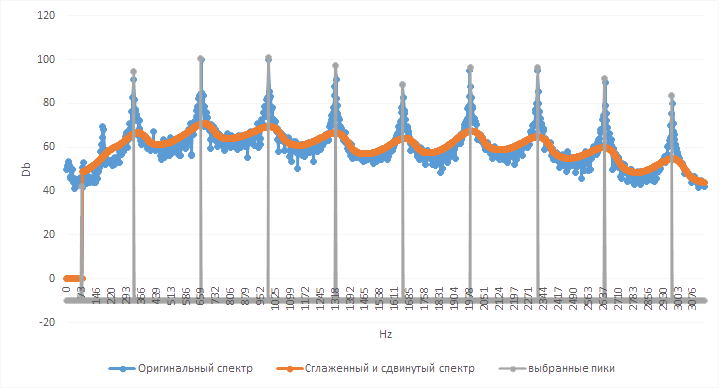
\includegraphics[width=0.45\textwidth]{img/spectre-guitar}\ \ \ 
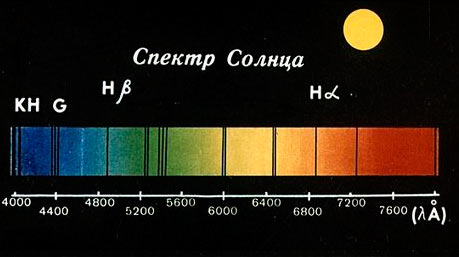
\includegraphics[width=0.45\textwidth]{img/spectre-sun}
\end{center}
\end{frame}

\section{scalar-prod}

\begin{frame} \frametitle{Как найти координаты?}
Перемножить сигнал и интересующую волну в каждой точке \\
и полученные значения сложить. \medskip

\centerline{
\includegraphics[width=0.6\textwidth]{img/sc_bigpos}}\vspace{-4mm}

Похожи~— сумма будет большая положительная. \medskip

\centerline{
\includegraphics[width=0.6\textwidth]{img/sc_bigneg}}\vspace{-4mm}

Ведут себя противоположным образом~— большая отрицательная. \medskip

\centerline{
\includegraphics[width=0.6\textwidth]{img/sc_orto}}\vspace{-4mm}

Совсем непохожи~— примерно 0.
\end{frame}

\section{show-stopper}


\begin{frame} \frametitle{\vspace*{-2.4cm}}
    \incg{python-fourier/signal}
\end{frame}

\begin{frame} \frametitle{\vspace*{-2.4cm}}
    \incg{python-fourier/waveform-2}

    \incg{python-fourier/fourier-2}
\end{frame}

\begin{frame} \frametitle{\vspace*{-2.4cm}}
    \incg{python-fourier/waveform-3}

    \incg{python-fourier/fourier-3}
\end{frame}

\begin{frame} \frametitle{\vspace*{-2.4cm}}
    \incg{python-fourier/waveform-5}

    \incg{python-fourier/fourier-5}
\end{frame}

\begin{frame} \frametitle{\vspace*{-2.4cm}}
    \incg{python-fourier/waveform-9}

    \incg{python-fourier/fourier-9}
\end{frame}

\begin{frame} \frametitle{\vspace*{-2.4cm}}
    \incg{python-fourier/waveform-15}

    \incg{python-fourier/fourier-15}
\end{frame}

\begin{frame} \frametitle{\vspace*{-2.4cm}}
    \incg{python-fourier/waveform-23}

    \incg{python-fourier/fourier-23}
\end{frame}

\begin{frame} \frametitle{\vspace*{-2.4cm}}
    \incg{python-fourier/waveform-25}

    \incg{python-fourier/fourier-25}
\end{frame}



\section{conclusion}

\begin{frame} \frametitle{\vspace*{-2.4cm}}
\begin{itemize}
	\item Преобразование Фурье раскладывает поступающий сигнал \\
	 в сумму волн фикс. частот с коэффициентами \medskip
	\item Полезно при сжатии данных (откинуть ненужные частоты),\\
	 при анализе сигнала \medskip
	\item Волны разных частот~— такой же {\bfseries\itshape ортогональный базис,}\\
	 как единичные векторы в пространстве. \bigskip
	\item А как {\bfseries\itshape быстро} считать это преобразование? \\
	 А что, если сигнал честно непрерывный? \\
	 {\bfseries\itshape А вот это уже интересно…}
\end{itemize} \bigskip

\begin{center}\Large\bf Спасибо за внимание! \end{center}
\end{frame}

\end{document}

\begin{frame} \frametitle{}
\end{frame}

\begin{nblock}{\vspace*{-3ex}}
	Sample text
\end{nblock}
